\begin{table}[H]
    \centering
	\begin{tabular}{lcccc}
	\textbf{Layer Type} & \textbf{Layer Config} & \textbf{Activation}  & \textbf{Output} & \textbf{Params}\\ \hline
	\conv	& \convP{5}{3}{5}	& relu		& \texttt{48,86,5} 	& \texttt{380}\\
	\flt		& /					& relu		& \texttt{20640}		& \texttt{0}\\
	\dns		& \dnsP{64}			& relu		& \texttt{64}		& \texttt{1321024}\\
	\dns		& \dnsP{6}			& softmax	& \texttt{64}		& \texttt{390}\\
	\multicolumn{4}{r}{\textbf{TOTAL}}&{\textbf{1,321,794}}\\
	\end{tabular}
	%Total params: 1,321,794
	%Trainable params: 1,321,794
	%Non-trainable params: 0
\end{table}

\begin{table}[H]
	\centering
	\begin{tabular}{lc}
	\textbf{Param} & \textbf{Value}\\ \hline
	Batch Size 	& 32 \\
	Optimizer 	& Adam \\
	Base lr		& 0.001 \\
	Epochs		& 20\\
	\end{tabular}
\end{table}


\begin{figure}[H]
	\begin{center}
	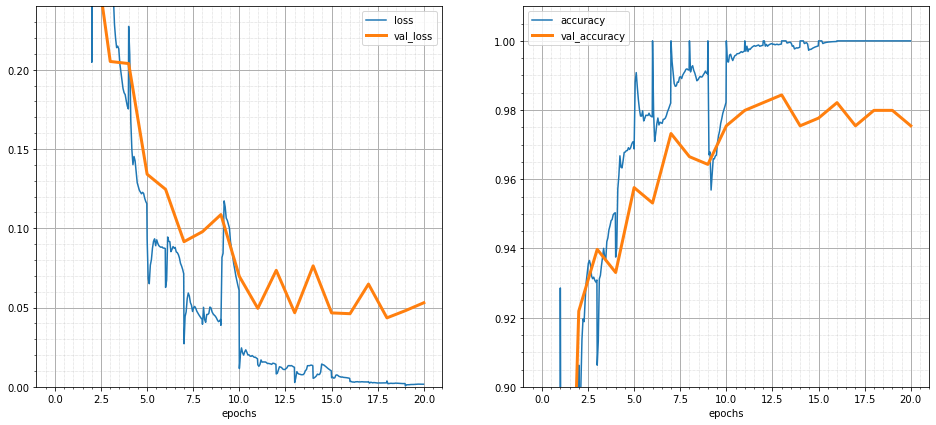
\includegraphics[width=\linewidth]{Immagini/Baseline-1}
	\caption{Graph of the first run}
	\end{center}
\end{figure}
\begin{table}[H]
	\centering
	\begin{tabular}{cccccc}
		\textbf{Run} &\textbf{Loss}&\textbf{V.Loss} &\textbf{Acc.}&\textbf{V.Acc.}&\textbf{$\Delta$ Acc.} \\ \hline
		1	& 0.0016		& 0.0530		& 1.0000		& 0.9754		& 0.0246 \\
		2	& 0.0012		& 0.0342		& 1.0000		& 0.9821		& 0.0179 \\
		3	& 0.0060		& 0.0497		& 0.9996		& 0.9866		& 0.0130 \\
		\textbf{Avg} & \textbf{0.0029}	& \textbf{0.0456}	& \textbf{0.9996} 	& \textbf{0.9814}	& \textbf{0.0185} 
	\end{tabular}
\end{table}

This is a very bare-bone, used to check everything is working in the net and to get a reference for the next iterations. Nevertheless, we can make a few observation:
\begin{itemize}
\item There is some overfitting occurring. This is due to the fact the image is only slightly reduced in the convolution, thereby creating the need for a substantial number of parameters between the flat layer and the first dense layer.
\item The training basically stall after the 10th epoch, as it has already reach maximum accuracy on the train dataset.
\end{itemize}

